\documentclass[aspectratio=169]{beamer}
\usepackage[T2A]{fontenc}
\usepackage[utf8]{inputenc}
\usepackage{xcolor,colortbl}
\usepackage{graphics}

\usepackage{tikz}
\usetikzlibrary{positioning,arrows.meta}

\usecolortheme{wolverine}
\definecolor{monerorange}{RGB}{255, 102, 0}
\definecolor{otherorange}{RGB}{253, 188, 148}
\definecolor{redd}{RGB}{253, 150, 179}
\definecolor{grenn}{RGB}{150, 253, 189}
\definecolor{yello}{RGB}{248, 253, 150}
\setbeamercolor*{palette primary}{bg=otherorange}
\setbeamercolor*{frametitle}{bg=otherorange}
\setbeamercolor*{itemize item}{fg=monerorange}
\setbeamercolor*{itemize subitem}{fg=monerorange}
\setbeamertemplate{footline}[frame number]

\newcommand{\com}{\operatorname{Com}}

\title{Triptych}
\subtitle{Логарифмически масштабируемые связываемые кольцевые подписи и их применение}
\author{Саранг Ноезер, кандидат технических наук}
\institute{Исследовательская лаборатория Monero}
\date{17 сентября 2020}
\begin{document}


\frame{\titlepage}


\begin{frame}{Цель}
Мы хотим построить схему \textbf{конфиденциальных транзакций}, обладающую следующими свойствами:
\begin{itemize}
\item не требующими доверия настройками и параметрами
\item сублинейным масштабированием размера в зависимости от размера анонимной группы
\item возможностью групповой верификации $O(n/\log(n))$
\item безопасной совместимостью с одноразовой адресацией
\item поддержкой выполнения операций с использованием мультиподписей
\end{itemize}
~\\
Наша схема называется \textbf{Triptych}.
\\~\\
Это результат совместной работы с \textbf{Брэндоном Гуделлом}.
\end{frame}


\begin{frame}{Наша стратегия}
\begin{center}
\begin{tikzpicture}[> = {Straight Barb[angle=60:4pt 6]}]
\node (general) {\underline{Общая структура}};
\node (rs) [draw, below=10pt of general] {RingSig};
\node (lrs) [draw, below=of rs] {Связываемая RingSig};
\node (2lrs) [draw, below=of lrs] {2-cвязываемая RingSig};

\node (monero) [right=50pt of general] {\underline{Протокол Monero}};
\node (schnorr) [below=10pt of monero] {SAG типа Шнорра};
\node (lsag) [below=of schnorr] {LSAG};
\node (clsag) [below=of lsag] {CLSAG/MLSAG};
\node (ringct) [draw, below=of clsag, align=center] {\textbf{Протокол кольцевых} \\ \textbf{конфиденциальных транзакций}};

\node (this) [right=60pt of monero] {\underline{\textbf{Данная работа}}};
\node (gkb) [below=10pt of this] {\textbf{Groth/Kohlweiss/Bootle}};
\node (triptych) [below=of gkb] {\textbf{Triptych}};
\node (2triptych) [below=of triptych] {\textbf{2-Triptych}};

\draw[->] (rs) to (lrs);
\draw[->] (lrs) to (2lrs);
\draw[->] (2lrs) to (ringct);

\draw[->,dashed] (schnorr) to (lsag);
\draw[->,dashed] (lsag) to (clsag);
\draw[->,dashed] (clsag) to (ringct);

\draw[->,dashed] (gkb) to (triptych);
\draw[->,dashed] (triptych) to (2triptych);
\draw[->,dashed] (2triptych) to (ringct);
\end{tikzpicture}
\end{center}
\end{frame}


\begin{frame}{Кольцевые подписи}
\textbf{Кольцевые подписи} является схемой подписи, используемой для подписания сообщения от лица \underline{неинтерактивной} анонимной группы, представленной публичными ключами. Подписанту известен секретный ключ (по крайней мере) к одному из публичных ключей, входящих в группу.
\\~\\
Верификатору известно, что только один из ключей в наборе публичных ключей принадлежит подписанту, но ему не известно, какой именно. Поэтому
$$\operatorname{Sign}(m,\{M_0,M_1,\ldots\};(l,r)) \to \sigma$$
подписывает сообщение $m$ так, что $M_l$ использует $r$ как секретный ключ и
$$\operatorname{Verify}(m,\{M_0,M_1,\ldots\},\sigma) \to \{0,1\}$$
верифицируется.
\end{frame}


\begin{frame}{Кольцевые подписи}
\begin{center}
\begin{tikzpicture}[
    box/.style = {draw, minimum width=30pt, minimum height=20pt, rounded corners, align=center},
    dot/.style = {draw, minimum width=30pt, minimum height=20pt, dashed, rounded corners, align=center},
    > = {Straight Barb[angle=60:4pt 6]}
]
\node (rs) [draw, minimum width=100pt, minimum height=40pt] {Кольцевая подпись};
\node (M1) [dot, left=of rs] {$M_1$};
\node (M0) [box, above=of M1] {$M_0$};
\node (M2) [box, below=of M1] {$M_2$};
\node (msg) [box, below=of rs] {сообщение};
\node (sig) [box, right=of rs] {$\sigma$};

\draw[-] (M0) to (M1);
\draw[-] (M1) to (M2);
\draw[->] (M1) to (rs);
\draw[->] (msg) to (rs);
\draw[->] (rs) to (sig);
\end{tikzpicture}
\end{center}
\end{frame}


\begin{frame}{Кольцевые подписи Groth/Kohlweiss/Bootle (GKB)}
В работе (IACR 2014/764) \textbf{Groth} и \textbf{Kohlweiss} предлагается новая система доказательства с нулевым разглашением, позволяющая построить схему кольцевой подписи. \textbf{Bootle} и его соавторы в своей работе (IACR 2015/643) описали более эффективный вариант этой системы.
\\~\\
Система предполагает построение сигма-протокола для отношения
$$\Big\{\{M_0,\ldots,M_{N-1}\};(l,r) : 0 \leq l < N, M_l = \com(0,r)\Big\}$$
для схемы обязательства $\com$, логарифмически масштабируемой по размеру относительно $N$.
\\~\\
Для преобразования в схему кольцевой подписи используется эвристический подход Фиата-Шамира и сообщение встраивается в хеш транскрипта.
\end{frame}


\begin{frame}{Свойства}
Неформально нам бы хотелось достичь нескольких полезных свойств. Они вытекают непосредственно из свойств лежащего в основе сигма-протокола.
\\~\\
\begin{itemize}
\item \textbf{Правильность}. Действительные подписи всегда будут верифицироваться.
\begin{itemize}
\item Полнота
\end{itemize}
\item \textbf{Анонимность}. Невозможность определения подписывающего индекса.
\begin{itemize}
\item Нулевое разглашение
\end{itemize}
\item \textbf{Невозможность подделки}. Невозможность формирования подписи без известного секретного ключа.
\begin{itemize}
\item (Особая) устойчивость
\end{itemize}
\end{itemize}
\end{frame}


\begin{frame}{Связываемые кольцевые подписи}
Что, если бы нам захотелось выявить двойное подписание безопасным способом?
\\~\\
\textbf{Связываемая кольцевая подпись} является кольцевой подписью, также обеспечивающей \underline{связываемость} подписи. Любые две действительные подписи, которые можно связать, используют один и тот же (неизвестный) секретный ключ. Таким образом,
$$\operatorname{Link}(\sigma,\sigma') \to \{0,1\}$$
позволяет определить, были ли две подписи подписаны одним и тем же секретным ключом.
\\~\\
Выбор анонимной группы может оказаться критически важным с точки зрения практической безопасности.
\\~\\
Можно создавать схемы, которые будут либо зависимы, либо независимы от анонимной группы.
\end{frame}


\begin{frame}{Связываемая кольцевая подпись Triptych}
Путём добавления свойства связываемости в схему GKB мы получаем \textbf{Triptych} (IACR 2020/018).
\\~\\
Это сводит сигма-протокол к отношению
$$\Big\{\{M_0,\ldots,M_{N-1}\}, J;(l,r) : 0 \leq l < N, M_l = \com(0,r), rJ = U\Big\}$$
с глобально постоянной $U$, где $J$ является \underline{связующим тегом}. Для проверки связываемости следует сравнить теги.
\\~\\
Для преобразования в схему кольцевой подписи используется эвристический подход Фиата-Шамира и сообщение встраивается в хеш транскрипта.
\end{frame}


\begin{frame}{Расширение схемы GKB до Triptych}
Возможно ли расширение схемы с GKB до Triptych? Обязательства по нулевой сумме следует рассматривать в качестве публичных ключей с групповым генератором $G$.
\\~\\
В случае с GKB мы доказываем знание $r$ таким образом, что некоторое обязательство будет иметь форму $rG = M$.
\\~\\
В случае с Triptych мы повторно используем некоторые из скрытых данных данного доказательства об $r$, чтобы показать, что $U$ соответствует форме $rJ = U$. Поскольку $U$ имеет глобально постоянное значение, доказывающая сторона может сделать это только в том случае, если укажет $J \equiv (1/r)U$, являющуюся верифицируемой случайной функцией.
\\~\\
Поскольку сигма-протокол является (особо) устойчивым и преобразование $r \mapsto J$ является биекцией, мы получаем свойство связываемости.
\end{frame}


\begin{frame}{2-связываемые кольцевые подписи}
Мы расширяем схему связываемой кольцевой подписи, чтобы продемонстрировать знание ключей в \underline{параллельных списках} публичных ключей.
\\~\\
Подписант даёт два списка публичных ключей и показывает, что ему известен секретный ключ к \underline{обоим} публичным ключам с \underline{одним и тем же} неизвестным индексом в обоих списках.
\\~\\
Таким образом, мы сохраняем свойство связываемости, но только для одного из списков (вскоре мы более подробно расскажем об этом)!
\end{frame}


\begin{frame}{2-связываемые кольцевые подписи}
\begin{center}
\begin{tikzpicture}[
    box/.style = {draw, minimum width=30pt, minimum height=20pt, rounded corners, align=center},
    dot/.style = {draw, minimum width=30pt, minimum height=20pt, dashed, rounded corners, align=center},
    > = {Straight Barb[angle=60:4pt 6]}
]
\node (rs) [draw, minimum width=100pt, minimum height=40pt, align=center] {2-связываемая \\ кольцевая подпись};
\node (M1) [dot, left=of rs] {$M_1$};
\node (M0) [box, above=of M1] {$M_0$};
\node (M2) [box, below=of M1] {$M_2$};

\node (P1) [dot, left=of M1] {$P_1$};
\node (P0) [box, above=of P1] {$P_0$};
\node (P2) [box, below=of P1] {$P_2$};

\node (msg) [box, below=of rs] {сообщение};
\node (sig) [box, right=of rs] {$\sigma$};

\draw[-] (M0) to (M1);
\draw[-] (M1) to (M2);
\draw[-] (M0) to (P0);
\draw[-] (M1) to (P1);
\draw[-] (M2) to (P2);
\draw[->] (M1) to (rs);
\draw[->] (msg) to (rs);
\draw[->] (rs) to (sig);
\end{tikzpicture}
\end{center}
\end{frame}


\begin{frame}{2-связываемые кольцевые подписи Triptych}
Мы изменяем Triptych, чтобы построить 2-связываемую кольцевую подпись; это даже можно сделать в более общем плане.
\\~\\
Это сводит сигма-протокол к отношению
\begin{multline*}
\Big\{\{M_0,\ldots,M_{N-1}\}, \{P_0,\ldots,P_{N-1}\}, J;(l,r,s) : \\
0 \leq l < N, M_l = \com(0,r), P_l = \com(0,s), rJ = U\Big\}
\end{multline*}
в которое теперь включены два списка публичных ключей.
\\~\\
Несмотря на то, что нам необходимы новые данные доказательства секретного ключа $s$, мы можем повторно использовать уже существующие данные доказательства по индексу $l$.
\end{frame}


\begin{frame}{Протокол кольцевых конфиденциальных транзакций}
Нам бы хотелось построить протокол \textbf{конфиденциальных транзакций}, который бы позволил:
\begin{itemize}
\item использовать множество выходов транзакций
\item генерировать множество выходов транзакций
\item скрывать суммы выходов
\item скрывать подписывающие индексы
\item поддерживать скрытую адресацию в сети
\end{itemize}
~\\
Мы можем сделать, используя произвольные 2-связываемые кольцевые подписи, такие как 2-Triptych или CLSAG.
\end{frame}


\begin{frame}{Протокол кольцевых конфиденциальных транзакций}
Определяем обязательство Педерсена $\com(v,r) \equiv vH + rG$ для групповых генераторов $G,H$.
\\~\\
Нам необходимо сгенерировать транзакцию, использующую $W$ существующих выходов и генерирующую $T$ новых выходов.
\\~\\
Формируем одиночную анонимную группу с $N \geq W$ публичных ключей $\{M_k\}_{k=0}^{N-1}$ так, чтобы для набора секретных индексов $\{l_u\}_{u=0}^{W-1} \subset [0,N)$ у нас было $M_{l_u} = r_uG$ для всех $0 \leq u < W$, где каждый $r_u$ являлся бы секретным ключом.
\end{frame}


\begin{frame}{Протокол кольцевых конфиденциальных транзакций}
Рассмотрим пример, где $W = 3$, а $N \geq 3$ являются произвольными.

\begin{center}
\begin{tikzpicture}
\node (M0) {$M_0$};
\node (M1) [right=of M0] {$M_1$};
\node (M2) [right=of M1] {$M_2$};
\node (dots) [right=of M2] {$\cdots$};
\node (MN1) [right=of dots] {$M_{N-1}$};
\node (r0) [below=of M2] {$r_0$};
\node (r1) [below=of M0] {$r_1$};
\node (r2) [below=of MN1] {$r_2$};

\draw[-, dashed] (r0) to (M2);
\draw[-, dashed] (r1) to (M0);
\draw[-, dashed] (r2) to (MN1);
\end{tikzpicture}
\end{center}

Таким образом, набором секретных индексов будет $\{l_u\}_{u=1}^{W-1} = \{2, 0, N-1\}$.
\end{frame}


\begin{frame}{Протокол кольцевых конфиденциальных транзакций}
Каждый из использованных выходов $0 \leq u < W$ связан с обязательством по сумме $a_u$:
$$P_{l_u} \equiv \com(a_u,s_u)$$

Поскольку система доказательства Triptych подразумевает знание обязательства по нулевой сумме, формируем \underline{офсет обязательства} для каждого использованного выхода с одинаковым значением, но единообразной случайной маской:
$$P'_u \equiv \com(a_u,s'_u)$$

Это сводит обязательства к нулю:
$$P_{l_u} - P'_u = \com(a_u,s_u) - \com(a_u,s'_u) = \com(0,s_u-s'_u)$$
\end{frame}


\begin{frame}{Протокол кольцевых конфиденциальных транзакций}
Генерируем $0 \leq j < T$ nновых выходов, где каждый имеет связанное с собой обязательство по суме (и доказательство диапазона):
$$Q_j \equiv \com(b_j,t_j)$$
Для $1 \leq j < T$ выбираем случайные маски $t_j$. Затем задаём
$$t_0 \equiv \sum_{u=0}^{W-1} s'_u - \sum_{j=1}^{T-1} t_j$$
так, чтобы верификатор смог произвести эту проверку, если соотношение использованных и новых выходов будет нормальным
$$\sum_{u=0}^{W-1} P'_u - \sum_{j=0}^{T-1} Q_j = 0$$
\end{frame}


\begin{frame}{Протокол кольцевых конфиденциальных транзакций}
Наконец, генерируем подпись для каждого из использованных выходов $0 \leq u < W$ , используя следующие входы отношения 2-Triptych:
$$\Big\{\{M_k\}_{k=0}^{N-1},\{P_k-P'_u\}_{k=0}^{N-1},(1/r_u)U; (l_u,r_u,s_u-s'_u)\Big\}$$
Чтобы верифицировать каждую транзакцию, необходимо:
\begin{itemize}
\item верифицировать каждую из связываемых кольцевых подписей
\item произвести тест на связываемость для всех подписей
\item выполнить успешную проверку правильности соотношения
\item верифицировать доказательства диапазона всех выходов
\end{itemize}
\end{frame}


\begin{frame}
\centering
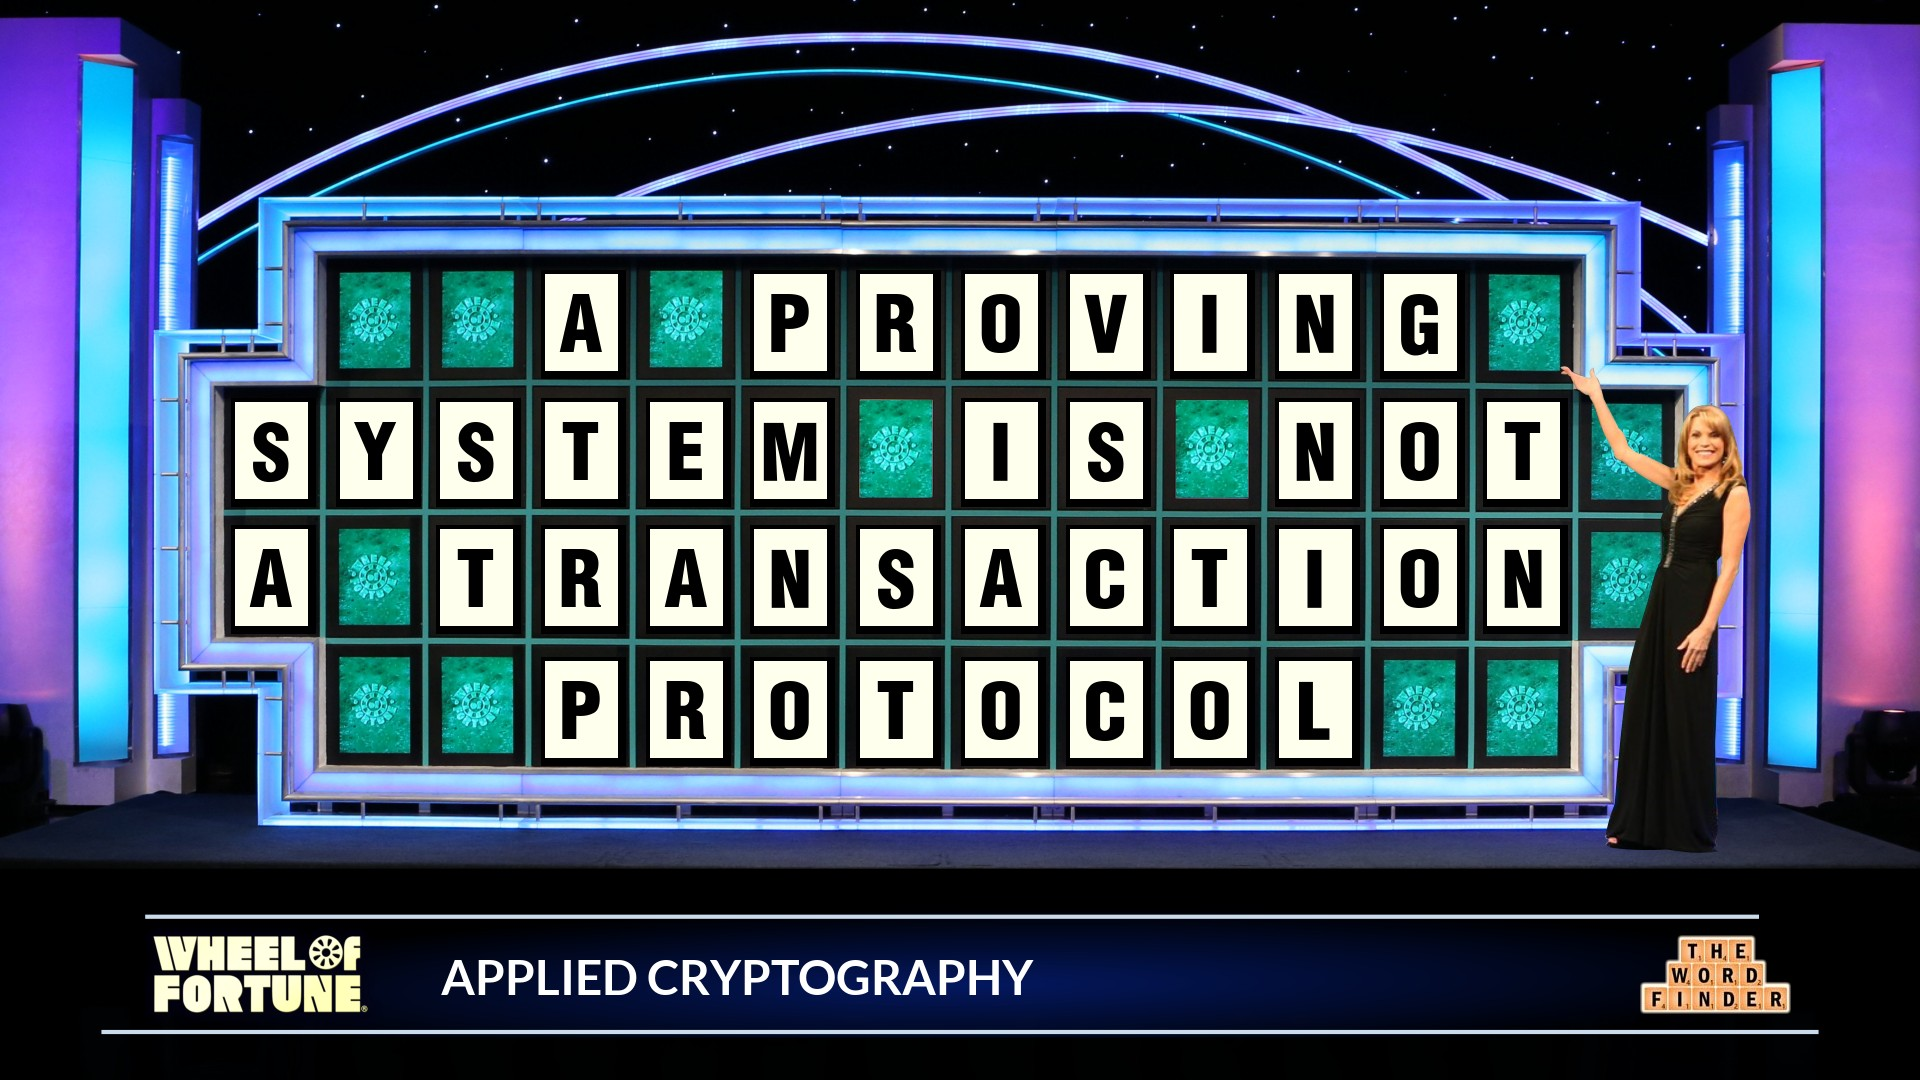
\includegraphics[width=\textwidth]{protocol.jpeg}
\end{frame}


\begin{frame}{Сравнение}
\begin{center}
\renewcommand{\arraystretch}{1.5}
\begin{tabular}{|r|ccccc|}
\hline
& Размер & Верификация & Группирование & Адресация & Накопление \\
\hline
\textbf{Triptych} & \cellcolor{grenn} $O(\log N)$ & \cellcolor{yello} $O(N/\log N)$ & \cellcolor{grenn} есть & \cellcolor{grenn} есть & \cellcolor{redd} нет \\
Arcturus & \cellcolor{grenn} $O(\log N)$ & \cellcolor{yello} $O(N/\log N)$ & \cellcolor{grenn} есть & \cellcolor{grenn} есть & \cellcolor{grenn} есть \\
CLSAG & \cellcolor{redd} $O(N)$ & \cellcolor{redd} $O(N)$ & \cellcolor{redd} нет & \cellcolor{grenn} есть & \cellcolor{redd} нет \\
Lelantus & \cellcolor{grenn} $O(\log N)$ & \cellcolor{yello} $O(N/\log N)$ & \cellcolor{grenn} есть & \cellcolor{redd} нет & \cellcolor{redd} нет \\
Omniring & \cellcolor{grenn} $O(\log N)$ & \cellcolor{yello} $O(N/\log N)$ & \cellcolor{redd} нет & \cellcolor{grenn} есть & \cellcolor{grenn} есть \\
RingCT 3.0 & \cellcolor{grenn} $O(\log N)$ & \cellcolor{yello} $O(N/\log N)$ & \cellcolor{grenn} есть & \cellcolor{grenn} есть & \cellcolor{yello} частично \\
\hline
\end{tabular}
\end{center}

\begin{center}
Данная таблица умышленно упрощена.
\end{center}
\end{frame}


\begin{frame}{Заключение}
\textbf{Triptych} вляется системой доказательства с нулевым разглашением, которая может использоваться для построения схемы связываемой (и 2-связываемой!) кольцевой подписи, которая, в свою очередь, может усилить модель конфиденциальных транзакций. Система:
\begin{itemize}
\item не требует доверенных настроек или параметров
\item масштабируется логарифмически по размеру (при этом увеличение размера зависит от рациональности используемого размера анонимной группы)
\item масштабируется (суб)-линейно во время верификации с возможностью группирования
\item полностью совместима со скрытой адресацией в сети
\item поддерживает выполнение операций с использованием мультиподписей посредством общего секрета Пэйе
\end{itemize}
\begin{center}
~\\
\textbf{\Large Вопросы?}
\end{center}
\end{frame}


\end{document}